\documentclass[handout]{beamer}
\usepackage{array}
\usepackage{german}
\usepackage{graphicx}
\usepackage[utf8]{inputenc}
\usepackage[T1]{fontenc}
\mode<beamer>{%
\usetheme{Copenhagen}
}
\usepackage[orientation=landscape,size=a3,debug,scale=2.9]{beamerposter}
\title[]{}
\begin{document}
\begin{frame}
\frametitle{MathSem 2018: Klimawandel}
\begin{columns}[onlytextwidth]
\begin{column}{0.32\textwidth}
{\bf\large Das Buch zum Seminar}
\bigskip
\vskip 1cm
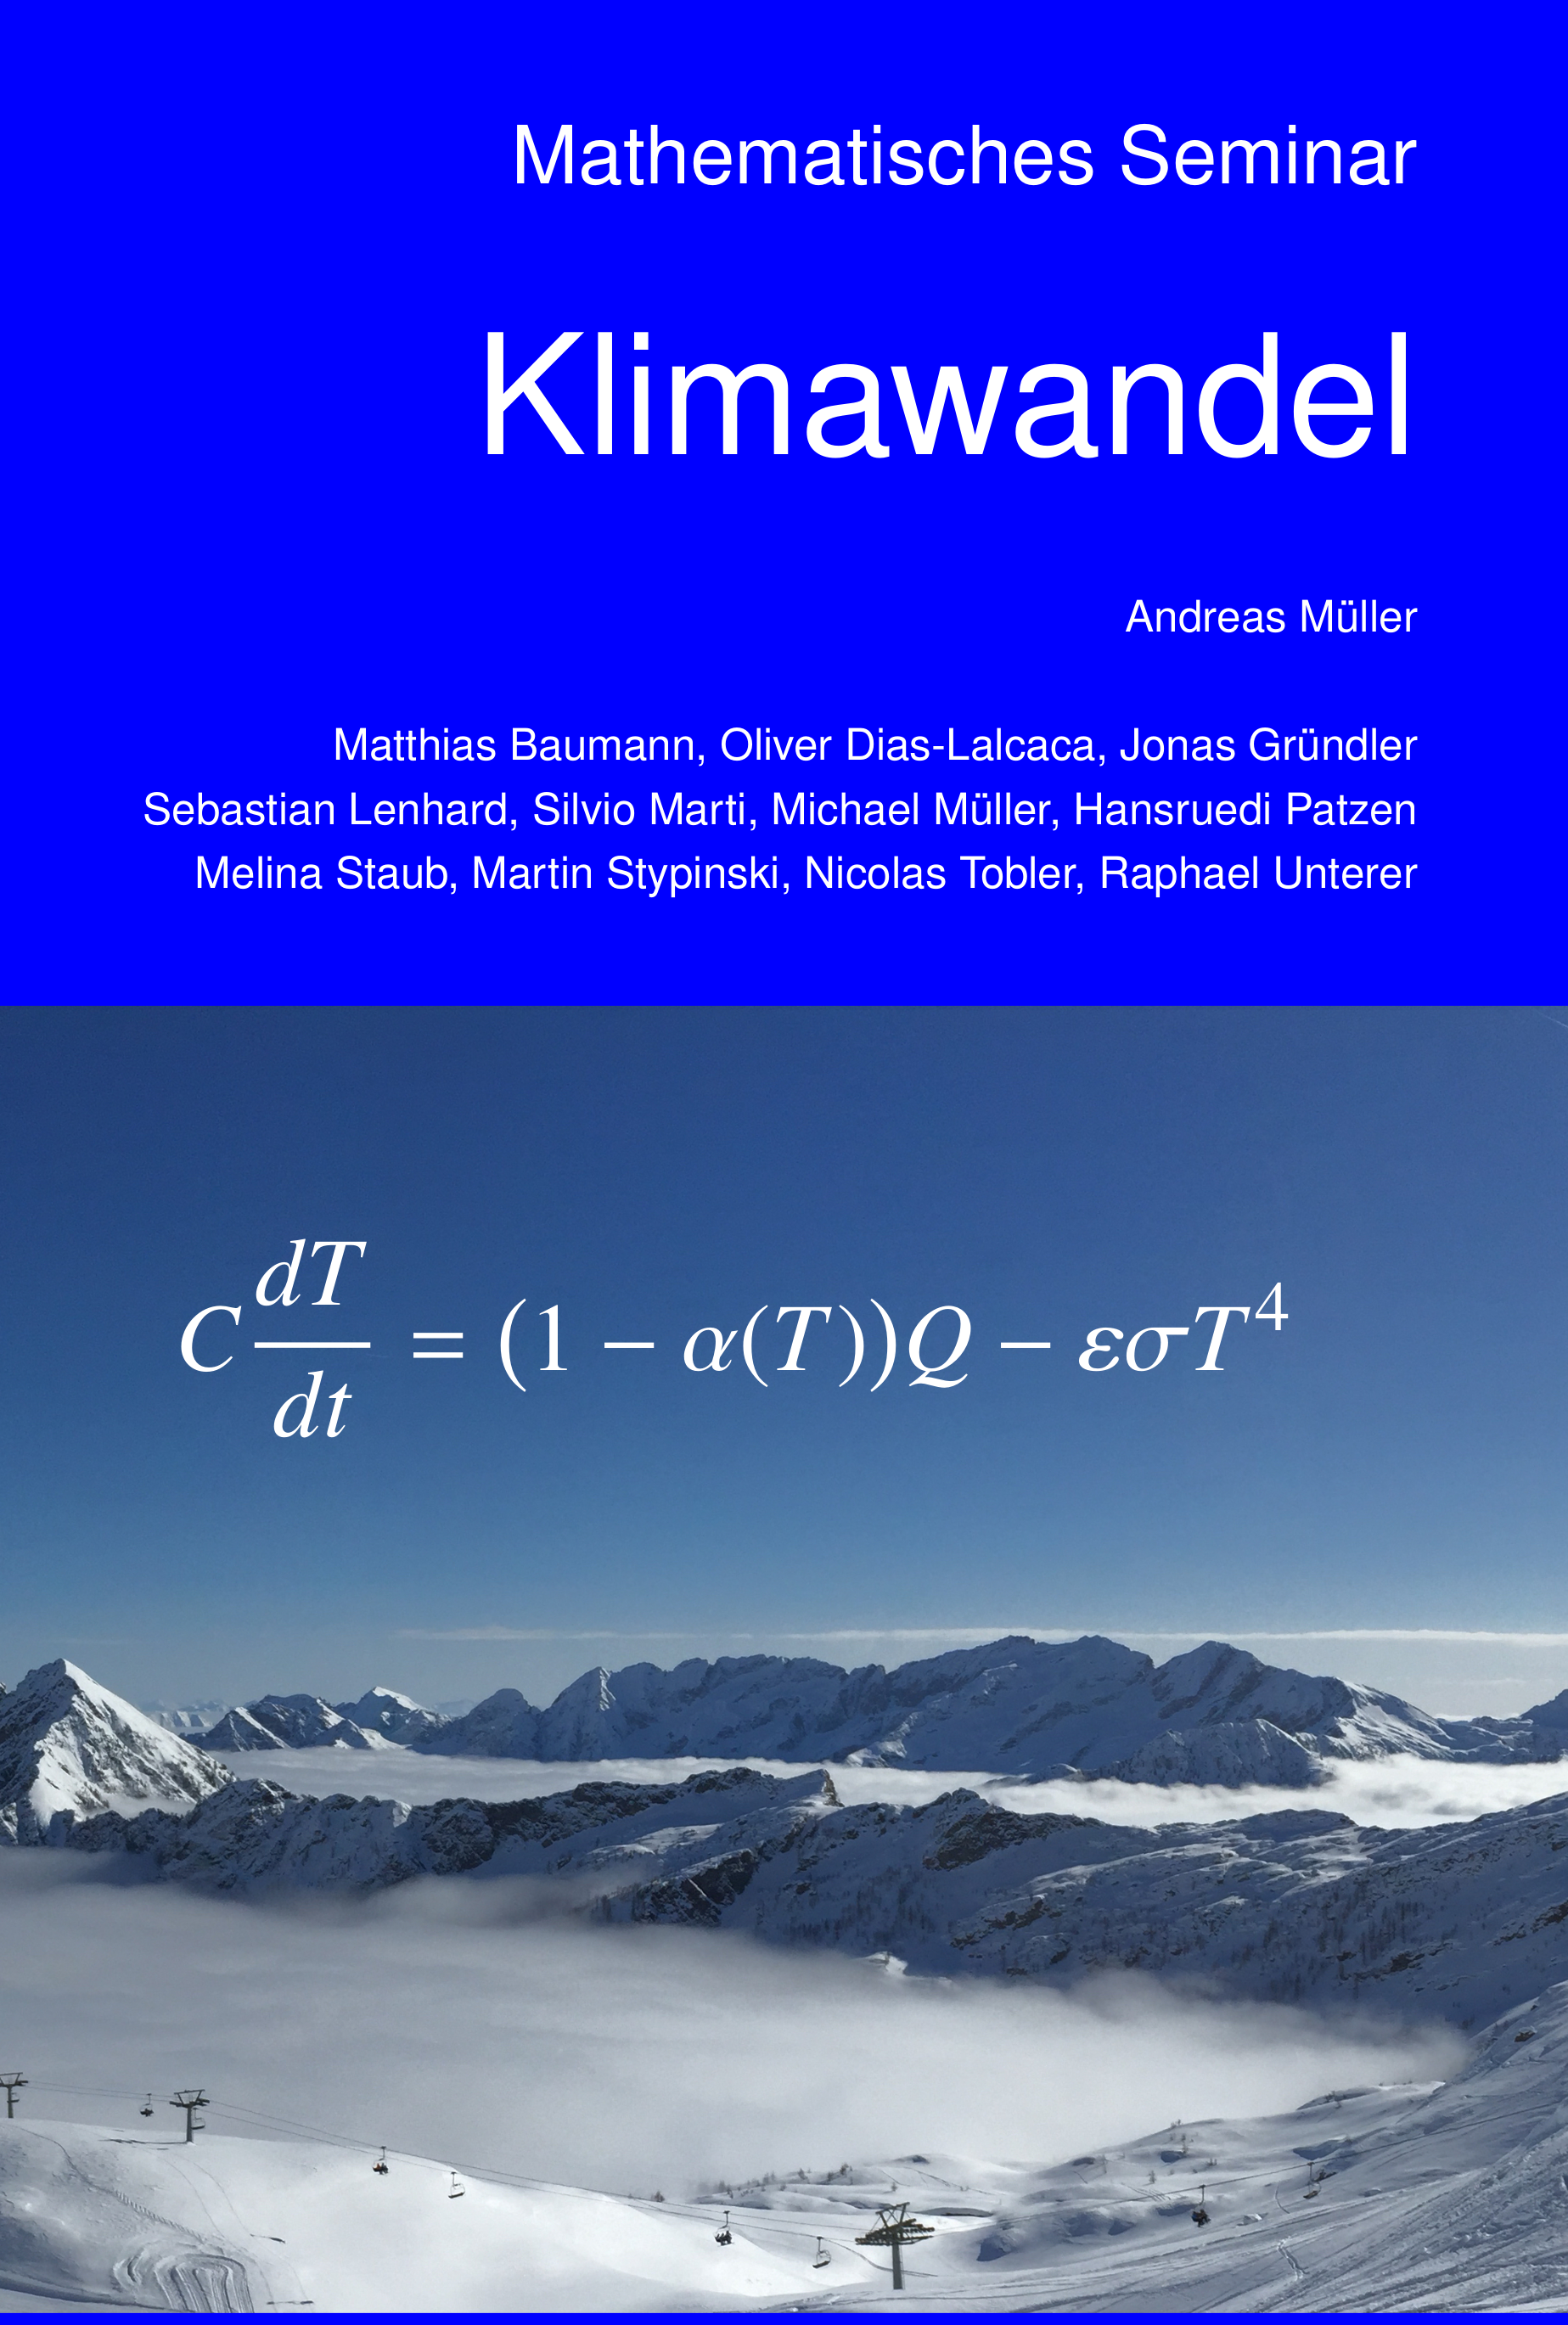
\includegraphics[width=\hsize]{cover-medium.png}
\vskip 0.2cm
%\bigskip
%\bigskip
%\bigskip
Erscheint im September 2018.
Anfragen an
Prof.~Dr.~Andreas M"uller,
{\texttt{andreas.mueller@hsr.ch}}
\end{column}
\begin{column}{0.63\textwidth}
\begin{description}
\item[Teil 1:] Grundlagen
\begin{enumerate}
\item Wetter und Klima
\item Differentialgleichungen
\item Fluiddynamik
\item Thermohaline Zirkulation
\item Zonenmodelle
\item Fourier-Analysis
\item El Niño Southern Oscillation
\item Datenassimilation
\end{enumerate}
\item[Teil 2:] Anwendungen und weiterführende Themen
\begin{enumerate}
\setcounter{enumi}{8}
\item Matthias Baumann und Oliver Dias: {\em Lorenz-Attraktor}
\item Hansruedi Patzen: {\em Höherdimensionales Lorenzsystem}
\item Martin Stypinski: {\em Machine Learning und Klimamodelle}
\item Jonas Gründler: {\em 3-Box-Modell der Thermohalinen Zirkulation}
\item Silvio Marti: {\em Eis}
\item Raphael Unterer: {\em Numerische Lösung einer verzögerten Differentialgleichung}
\item Nicolas Tobler: {\em Klima auf anderen Planeten}
\item Sebastian Lenhard: {\em Achsneigung und Eiszeiten}
\item Michael Müller: {\em Datenassimilation für das Lorenz-System}
\item Melina Staub: {\em Extreme Ereignisse}
\end{enumerate}
\end{description}
\end{column}
\end{columns}
\end{frame}
\end{document}
